% SVN info for this file
\svnidlong
{$HeadURL$}
{$LastChangedDate$}
{$LastChangedRevision$}
{$LastChangedBy$}

\chapter{Overview of HIL and BMI}
\labelChapter{Chapter_1}

\begin{introduction}
  This chapter will describe from the ground up the overall HIL and BMI ecosystem and how it fits into the MOC.
\end{introduction}


\section{What is MOC, HIL and BMI?}

\lettrine[nindent=-1pt]{T}{he key idea behind the Massachusetts Open Cloud (MOC)} is to operate based on an \index{Open Cloud eXchange (OCX)}Open Cloud eXchange (OCX) model, where multiple stakeholders provide one or more services rather than just one cloud provider.  This requires one to have more control over the provided resources --- such as nodes and switches --- via projects such as the \index{Hardware Isolation Layer (HIL)}\emph{Hardware Isolation Layer (HIL)} for \index{network isolation}network isolation of nodes, and the \index{Bare Metal Imaging (BMI)}\emph{Bare Metal Imaging (BMI)} project for advertising (provisioning) to nodes, images to boot from.  The key idea behind BMI is to provision and reprovision nodes with images quickly as demand for compute nodes (and resources) shifts between the Cloud and high-performance computing (HPC) jobs.  \\ %with. \\

The general idea is that we want many users (\index{multi-tenancy}\emph{multi-tenancy}) to have \emph{cloudlets} of nodes on isolated networks from other users running specific images.  The reason for the bare-metal approach is that is much faster than the virtual-machine approach for obvious reasons (i.e. hypervisor versus direct-hardware for booting and memory-management, etc).


\section{Network Isolation}

The first step that takes place in this process is the isolation of nodes.  All the nodes that are available for imaging are connected to a \emph{switch}.  Among them some will be in use by other users and some are free for use, or in the \emph{free pool} of available nodes.  \\

Every node is connected to a port on a switch.  A port is a physical connection between the node and the switch.   Switches operate on the \emph{\emph{data link layer (layer 2)}} of the OSI model.  If one would like to take a set of free nodes and isolate them on their own network, you would assign them to a \index{Virtual LAN (VLAN)}\emph{Virtual LAN (VLAN)}.  Assigning nodes to a VLAN simply means assigning the ports on that switch a number between 1 - 4096, which is the maximum number of VLANs possible.  So if you want 3 nodes and the VLAN 19 is available, you write to those ports using the software for that switch (i.e. Cisco or DELL at MOC) that value.  In fact, if you want a node to see other networks, you can assign the port that the node is attached to multiple VLAN numbers.  So think of each port on the switch having assigned a set of VLAN numbers --- and since VLANs are a broadcast domain --- then it can see any other ports (i.e. nodes) that intersect the set of assigned VLANs.  Each Ethernet packet has 12 bits allocated to store its VID (\index{VLAN ID}VLAN ID).  Below is an example of a switch with assigned ports: \\

$$
\begin{tabular}{|c|c|c|c|c|c|c|}
\hline

1 : \{ 19 \} & 2 : \{ 19 \} & 3: \{ 19, 20 \} & 4: \{ 20 \} & 5: \{ 20 \} & 6: \{\} & 7: \{ 20 \}  \\
\hline 
8 : \{ 19 \} & 9 : \{ 19 \} & 10: \{\} & 11: \{\} & 12: \{\} & 13: \{\} & 14: \{\}  \\
\hline
\end{tabular}
$$

\text{} \\

You will notice that nodes $1, 2, 3, 8,$ and $9$ are on VLAN $19$, while nodes $3, 4, 5,$ and $7$ are on VLAN 20 --- with all other nodes being unassigned (i.e. in the free pool of nodes).  Notice that node 3 will see all the nodes on both VLANs as it is assigned both VLAN numbers.  Thus if you want to have a public network you would assign it the same VLAN number to all the ports on the switch.  In fact, you can connect two switches which is referred to as \index{trunking}\emph{trunking} and those ports that connect switches would need to be assigned \emph{all} the numbers on both switches so that they are reachable.  \\

This is isolation of networks is basically what \index{HIL}HIL performs.  Since VLAN numbers are not natural to remember, they are aliased via a name that HIL refers to as the \emph{network}.  Thus one VLAN number will have a unique network name.  Users typically now just create an isolated network via HIL, and then come to BMI to \index{provision}\emph{provision} (assign images) to those nodes.  Next I will describe how BMI works.

\section{Bare Metal Imaging (BMI)}

Now you have a network name you created via HIL, and the nodes (using the name of NIC [Network Interface Controller]) that belong to that network.  Remember each node is connected to a NIC (port).  Now what you are interested is to boot those nodes, and somehow they find the images they should boot with.  How can that be done? \\

The general boot process of a node, is as follows: \\

\begin{enumerate}

\item A node remote boots to a computer (via PXE booting). The \index{Preboot Execution Environment (PXE)}\emph{Preboot Execution Environment (PXE)} protocol, allows one to boot a node using an image available on a remote \index{DHCP}DHCP server. \\

\item The image on that remote DHCP server --- in the case of BMI --- is actually an iPXE image, which enables one to see remote storage locations that contain larger bootable images.  iPXE allows one to use the iSCSI protocol (SCSI over Internet) in order to boot these images.  This process is called PXE $\rightarrow$ iPXE chainloading.

\end{enumerate}

\text{} \\

Basically BMI --- which we currently we run through a VM --- is just a gateway that services DHCP --- and other protocols required for PXE/iPXE --- only advertises bootable images available on remote network storage locations.  \textbf{\emph{Only HIL}} can \index{power-cycle the nodes}power-cycle the nodes so that they start the initiation process of looking for the DHCP server via PXE --- which can be called via the following REST request: \\

 \code{haas node\_power\_cycle NIC\_NAME } \\
 
\noindent  The power-cycle is performed via a separate \index{IPMI}IPMI\footnote{\link{https://en.wikipedia.org/wiki/Intelligent_Platform_Management_Interface}} \index{Intelligent Platform Management Interface (IPMI)}\emph{(Intelligent Platform Management Interface)} card, which is not visible by the operating system (OS) on the node but can be accessed separately - known as \index{out-of-band management (OOBM)}out-of-band management - to turn the machine on (i.e. power-cycle).  

\subsection{Preboot Execution Environment (\index{PXE}PXE) Protocol}

In the BIOS of any node, one sets the boot order of how that node should start up.  One of the settings is called \index{Preboot Execution Environment (PXE)}\emph{Preboot Execution Environment (PXE)}\footnote{\link{http://www.pix.net/software/pxeboot/archive/pxespec.pdf}}.  This basically performs a network boot using an image serviced from another location.  Here is how it happens: \\

\begin{enumerate}

\item The first thing that happens is that the PXE-enabled node broadcasts a \index{DHCPDISCOVER}DHCPDISCOVER request for an IP address from any computer on the network that runs a DHCP server.

\item Then the DHCP server sends back a list of Boot Servers.

\item Then the node discovers a Boot Server from that list and receives the name of an executable file on the Boot Server, which is the bootstrap file.

\item The node then uses the \index{Trivial FTP}\emph{Trivial FTP} protocol to download the executable file from the Boot Server.

\item The node will initiate the execution of that downloaded image.

\end{enumerate}

\text{} \\

Now the next step in the process is to perform an \index{iPXE}iPXE boot, which will again request an IP address from a DHCP server, but will this time boot a specific image from a remote network storage location. \\ 

\subsection{Advertising iSCSI Targets}

\index{SCSI}SCSI is a bus architecture that uses a protocol to interface via an \index{initiator}\emph{initiator} connecting multiple \index{targets}\emph{targets}.  On a computer the initiator is a controller card with multiple devices being the targets.  Over IP the initiator sends SCSI commands over the network treating the storage as if it were directly attached. \\

With BMI we use a package called \emph{Linux SCSI target framework (tgt)}, which can be accessed at the following link: \link{http://stgt.sourceforge.net/} \\

Currently we use \emph{Ceph} (\link{http://ceph.com/}) as our distributed storage system.  \index{Ceph}Ceph is an object storage implementation that implemented as a \emph{reliable autonomic distributed object store (RADOS)}.  These objects are accessible via a \index{RADOS Block Device (RBD)}\emph{RADOS Block Device (RBD)}, which we configure our \index{TGT}TGT iSCSI target images through.  To isolate the BMI development environment images in Ceph, we have a pool called \emph{boot-disk-prototype}.  In our implementation, the BMI service contains the initiator and the targets, which communicates via RBD to Ceph.\\

Since BMI performs the advertising of iSCSI targets, that is configured via files located in the \code{/etc/tgt/conf.d/} directory.  Below is an example of a file called \code{hadoop\_image-target.conf}: \\

%\pagebreak

\code{
<target pg-test> \\
\text{}\hspace{12mm}    driver iscsi \\
\text{}\hspace{12mm}    bs-type rbd \\
\text{}\hspace{12mm}    backing-store boot-disk-prototype/hadoop\_image \\
\text{}\hspace{12mm}    bsopts ""conf=/etc/ceph/ceph.conf;id=henn"" \\
\text{}\hspace{12mm}    write-cache off \\
\text{}\hspace{12mm}    initiator-address ALL \\
\text{}\hspace{8mm}</target>
}

\text{} \\

The above will configure the target called \code{hadoop\_image} The next step is to run the following command: \\

\code{tgt-admin -{}-execute} \\

\noindent which will advertise the image.  To see the target advertised you can just type the following: \\

\code{tgt-admin -s} \\

\noindent and you will begin to see something as follows: \\

\code{
Target 1: hadoop\_image \\
\text{}\hspace{12mm}    System information: \\
\text{}\hspace{18mm}        Driver: iscsi \\
\text{}\hspace{18mm}        State: ready \\
\text{}\hspace{12mm} ... \\
}

The next step is to configure the PXE file for the specific node defined by its NIC's MAC address, such as \code{/var/lib/tftpboot/pxelinux.cfg/01-90-e2-ba-9f-90-b0}, that might look as follows: \\

\code{
DEFAULT menu \\
\text{}\hspace{12mm}   PROMPT 0 \\
\text{}\hspace{12mm}   MENU TITLE PXE Menu \\
\text{}\hspace{12mm}   TIMEOUT 30 \\
\text{}\hspace{12mm}   ONTIMEOUT hadoop\_image \\
\text{} \\
\text{}\hspace{6mm} LABEL hadoop\_image \\
\text{}\hspace{12mm}      MENU LABEL hadoop\_image \\
\text{}\hspace{12mm}      KERNEL ipxe.lkrn \\
\text{}\hspace{12mm}      INITRD cisco-05.ipxe \\
}

The iPXE file would also need to be updated -- which is named based on the NIC as somthing like \code{/var/lib/tftpboot/cisco-05.ipxe} -- and would look as follows: \\

\code{
\#!ipxe \\
\text{}\hspace{12mm}      set keep-san 1 \\
\text{}\hspace{12mm}      ifconf --configurator=dhcp net2 \\
\text{}\hspace{12mm}      sanboot --keep iscsi:192.168.29.23:tcp:3260:1:hadoop\_image \\
\text{}\hspace{12mm}      boot \\
}      

Basically now the image is advertised and all that is necessary is for the node to be powered on.  When that happens it will automatically discover this DHCP server, which will start the process of pointing it to the correct image.  This is basically what BMI does, with the additional step of cloning the image so that the original golden image remains pristine.   Below is the general workflow of BMI: \\

\begin{figure}[!h] % Example of including images
\begin{center}
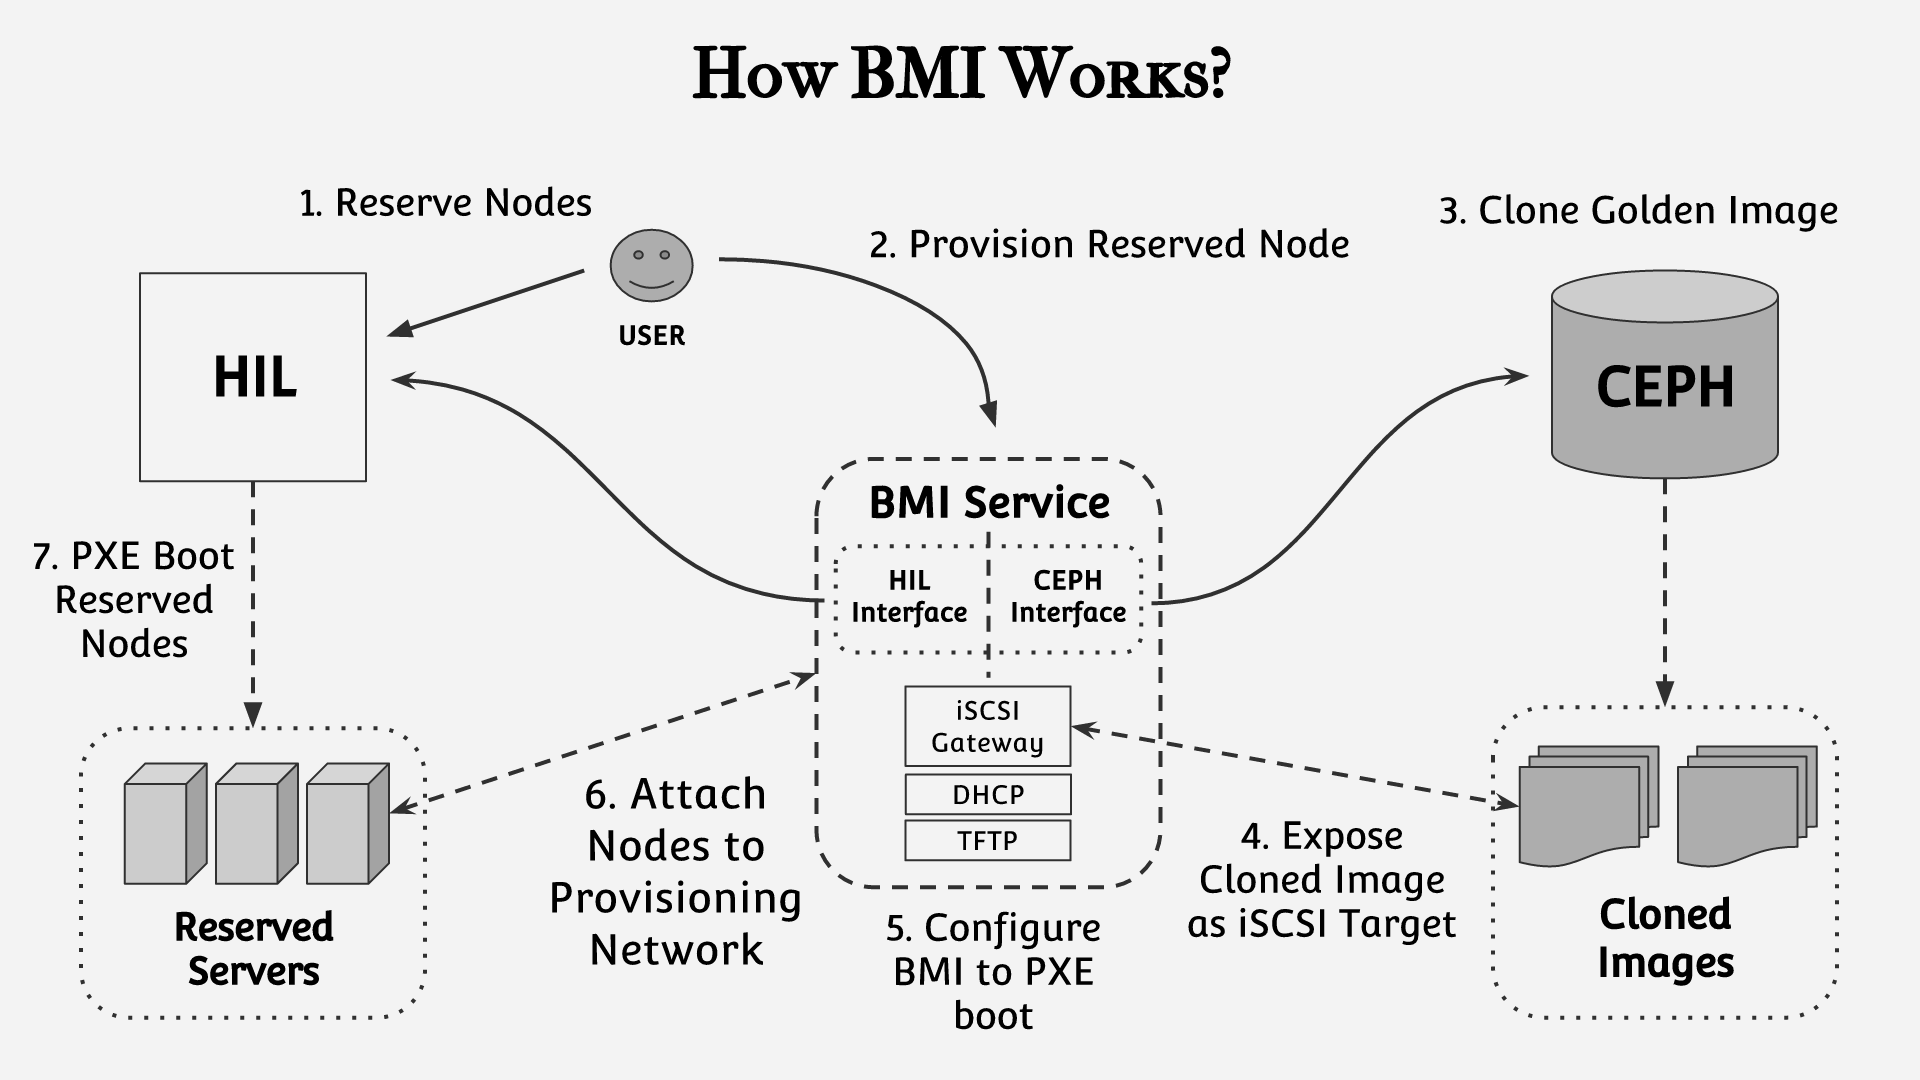
\includegraphics[scale=0.21]{figures/BMIFLOW.png}
\end{center}
\caption{HIL and BMI Ecosystem}
\label{fig:bmi-ecosystem}
\end{figure}



%\pagebreak \noindent 
It is important to understand that each node has a IPMI network card, and additional regular network cards.  The \index{IPMI network card}IPMI network card is isolated from the operating system (OS) of the machine, and can be remote-managed via the \emph{ipmi-tools}.  The process of booting is in two steps via a chainloading from PXE to iPXE, both of which will perform broadcast requests for DHCP IP addresses.  The \emph{haas-master (HIL)} will need to be on the same isolated network as the BMI service (VM).  The node that the BMI service is running on has the DHCP and TFTP services running on the same machine.  During the iPXE boot process, the Ceph storage location will be used to for booting the remote image, and all remote images (including golden standard ones) will initiate a snapshot delta-difference for storing the changes that one will make while using the image remotely on a node.  The remote boot process is performed via the iSCSI protocol. \\







\section{Communication Protocols for BMI}

Every BMI command is implemented as a \index{REST service}REST service.  The REST request can then be transformed into RPC calls, which are mapped to functions performing the BMI commands.  The architecture is as follows: \\

\begin{figure}[!h] % Example of including images
\begin{center}
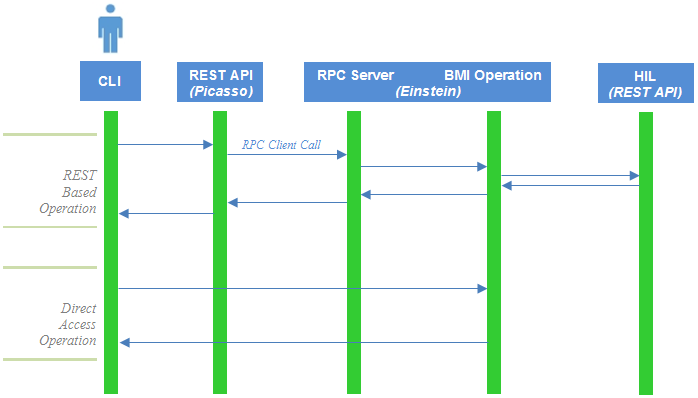
\includegraphics[scale=0.8]{figures/rest-rpc-bmi-calls-more-arrows-v2.png}
\end{center}
\caption{The REST and RPC call architecture of BMI}
\label{fig:bmi-rest-rpc-architecture}
\end{figure}

The user will interact via a \emph{command-line interface (CLI)}.  The calls are shaped as REST calls, which are serviced by the \emph{Picasso} server, which will propagate the call via \index{RPC calls}RPC calls that are exposed via the \emph{Einstein} server.  The Picasso service uses Flask\footnote{\link{http://flask.pocoo.org/}}  as its REST implementation, with Pyro\footnote{ \link{https://pythonhosted.org/Pyro4/}} to expose BMI functions through RPC calls.  Some calls are made via the REST service (i.e. provisioning a node), while others are made directly via BMI function-calls (i.e. listing the imported images). %  which communicates via RPC calls 


\subsection{REST API (\index{Picasso}Picasso)}

An overview of the REST API is available at the following link:

\begin{center}
  \link{https://github.com/CCI-MOC/ims/blob/dev/docs/rest_api.md}
\end{center}

%\pagebreak

Picasso's REST service implementation is available at the following link:

\begin{center}
  \link{https://github.com/CCI-MOC/ims/blob/dev/ims/picasso/rest.py}
\end{center}

Picasso will instantiate a RPC client that interfaces with Einstein's RPC server.  The RPC client is defined at the following link:

\begin{center}
  \link{https://github.com/CCI-MOC/ims/blob/dev/ims/rpc/client/rpc_client.py}
\end{center}


The RPC server code is defined at the following link:

\begin{center}
  \link{https://github.com/CCI-MOC/ims/blob/dev/ims/rpc/server/rpc_server.py}
\end{center}

%\noindent 
This then calls the appropriate \emph{BMI} operation method in Einstein.




\subsection{BMI Operations (\index{Einstein}Einstein)}

The main file that performs all the BMI operations is defined in the following file: %called from \emph{Picasso} is defined in the following file:

\begin{center}
  \link{https://github.com/CCI-MOC/ims/blob/dev/ims/einstein/operations.py}
\end{center}

In order to preserve a state, BMI instantiates a database.  All database entries are performed during the operations phase. \\

\section{BMI Configuration}

BMI gets configured at startup via a call to the instantiation of the \emph{\code{BMIConfig}} class, defined in the \code{config.py} file:

\begin{center}
\link{https://github.com/CCI-MOC/ims/blob/dev/ims/common/config.py}
\end{center}


This instantiation consumes the path of the location of the config file, which resides in either an environmental variable called \code{BMI\_CONFIG}, or in a file.  The default location of the config file's path  is defined by the \code{CONFIG\_DEFAULT\_LOCATION}, instantiated in the following file:

\begin{center}
\link{https://github.com/CCI-MOC/ims/blob/dev/ims/common/constants.py}
\end{center}


\section{Boot Order of a Node}

The boot order for BMI is performed in the following order: \\
\begin{enumerate}
  \item BIOS is set to \emph{Network Boot} (i.e. PXE). \vspace{3mm}
  \item The NIC performs DHCP request to the BMI Server, which has the DHCP server running.  The configuration for BMI is performed via PXELINUX which is a Syslinux\footnote{\link{http://www.syslinux.org/wiki/index.php?title=PXELINUX}} derivative. \vspace{3mm}
  \item In response, the DHCP server will reply with an IP address and bootfile specified as \code{pxelinux.0}.  After \code{pxelinux.0} get booted on the node, it will search on the BMI service the configured \emph{mac.temp} file\footnote{\text{}\hspace{1mm}The search-order is defined at the following link: \\ \text{}\hspace{7mm}\link{http://www.syslinux.org/wiki/index.php?title=PXELINUX\#Configuration}} as the second option -- which will be named as the node-specific MAC-address.  For PXELINUX, the \emph{mac.temp} file will be saved under the \code{/var/lib/tftpboot/pxelinux.cfg/} directory -- configured via BMI's \code{operations.py} file -- as the MAC address of the node\footnote{\text{}\hspace{1mm}An example of MAC-address-associated filename is:\\ \text{}\hspace{8mm}\code{/var/lib/tftpboot/pxelinux.cfg/01-90-e2-ba-9f-90-b0}}.  This template file is available here\footnote{\text{}\hspace{1mm}The Syslinux configuration standard is defined at the following link:\\
\text{}\hspace{7mm}\link{http://www.syslinux.org/wiki/index.php?title=Config}}:  

\begin{center}  
  \link{https://github.com/CCI-MOC/ims/blob/dev/ims/mac.temp}
\end{center}  

That file will contain the configured iPXE boot configuration via the following file, which will contain the exposed iSCSI target containing the CEPH image (or snapshot):

\begin{center}  
  \link{https://github.com/CCI-MOC/ims/blob/dev/ims/ipxe.temp}
\end{center}  

The boot process will be \textbf{\emph{chainloaded}} via PXE ($\rightarrow$ DHCP) $\rightarrow$ iPXE ($\rightarrow$ DHCP) to the iSCSI target all peformed via TGT or IET \footnote{\link{http://iscsitarget.sourceforge.net/}} \emph{(iSCSI Internet Target)}.  TGT has ACL and multi-tennancy in user-space.  IET performs this in kernel-space.  The \emph{ipxe.lkrn} file will be downloaded and loaded as a \emph{ramdisk}, which has been compiled once at the beginning of the BMI installation. \\ %This file gets provided by \emph{Picasso}. 

\end{enumerate}

In the next chapter, you will have a chance to work with BMI, in order to learn how to use its features.